\begin{theorem}[Triangle Inequality]
	\label{nprop:t:triangle}
	For all numbers $a$ and $b$, we have
	$$
		|a + b| \leq |a| + |b|.
	$$
\end{theorem}

%-------------------------------------------------------------------------------------------------------------
\begin{axiom}[Not in the book] %% 1.2
	\label{nprop:a:sqrt}
	For any $y \geq 0$, there is some $x \geq 0$ such that $x^2 = y$.
\end{axiom}

\Newpage
%-------------------------------------------------------------------------------------------------------------
\begin{restatable}[Not in the book]{lemma}{npropSqrtL} %% 1.3
	\label{nprop:l:sqrt}
	For any $y \geq 0$, there is a unique $x \geq 0$ such that $x^2 = y$. We denote $x = \sqrt{y}$.
\end{restatable}

\begin{proof}
	Let $y \geq 0$. By Axiom \ref{nprop:a:sqrt} we see that there is some $x \geq 0$ such that $x^2 = y$. Let $z \geq 0$, and suppose that $z^2 = y$. Then $z^2 = x^2$. If either $x = 0$ or $z = 0$, then clearly $z = x$. Now suppose that $x \neq 0$ and $z \neq 0$. Then,
	\begin{align*}
		z^2 = x^2 & \iff z z = x x                                   \\
		          & \iff (z z)(x^{-1} z^{-1}) = (x x)(x^{-1} z^{-1}) \\
		          & \iff (z x^{-1})(z z^{-1}) = (x z^{-1})(x x^{-1}) \\
		          & \iff z x^{-1} = x z^{-1}.
	\end{align*}
	Because $x > 0$ and $z > 0$, we deduce that $x^{-1} > 0$ and $z^{-1} > 0$, so $x^{-1} + z^{-1} > 0$. We also know that $x x^{-1} = 1 = z z^{-1}$. Then,
	\begin{align*}
		z x^{-1} & + z z^{-1} = x z^{-1} + x x^{-1}               \\
		         & \iff z (x^{-1} + z^{-1}) = x (z^{-1} + x^{-1}) \\
		         & \iff z = x.
	\end{align*}
\end{proof}


\Newpage
\npropSqrtL*
%-------------------------------------------------------------------------------------------------------------
\begin{restatable}[Not in the book]{lemma}{npropSqrtMultL} %% 1.4
	\label{nprop:l:sqrt_mult}
	Let $x \geq 0$ and $y \geq 0$. Then $\sqrt{x y} = \sqrt{x} \sqrt{y}$.
\end{restatable}

\begin{proof}
	Using Lemma \ref{nprop:l:sqrt} we deduce that
	\begin{align*}
		x y = x y & \iff \sqrt{x y} \sqrt{x y} = \left( \sqrt{x} \sqrt{x} \right) \left( \sqrt{y} \sqrt{y} \right) \\
		          & \iff \sqrt{x y} \sqrt{x y} = \left( \sqrt{x} \sqrt{y} \right) \left( \sqrt{x} \sqrt{y} \right) \\
		          & \iff \left( \sqrt{x y} \right)^2 = \left( \sqrt{x} \sqrt{y} \right)^2                          \\
		          & \iff \sqrt{x y} = \sqrt{x} \sqrt{y}.
	\end{align*}
\end{proof}


\addtocounter{problem}{12}
\Newpage
%-------------------------------------------------------------------------------------------------------------
\begin{problem} %% 1.13
	\label{nprop:p:13}
	The maximum of two numbers $x$ and $y$ is denoted by $\max(x, y)$. Thus $\max(-1,3) = \max(3,3) = 3$ and $\max(-1,-4) = \max(-4,-1)= -1$. The minimum of $x$ and $y$ is denoted by $\min(x, y)$. Prove that
	\begin{align*}
		\max(x, y)  & = \frac{x + y + |y - x|}{2}, \\
		\min (x, y) & = \frac{x + y - |y - x|}{2}.
	\end{align*}
	Derive a formula for $\max(x, y, z)$ and $\min(x, y, z)$, using, for example
	$$
		\max(x, y, z) = \max(x, \max(y, z)).
	$$
\end{problem}

\begin{proof}
	Without loss of generality, suppose that $y \geq x$. Then $y - x \geq 0$ and $|y - x| = y - x$. We also deduce that $\max(x, y) = y$, so
	\begin{align*}
		2 \max(x, y) & = 2 y = y + y = (y + 0) + y                    \\
		             & = (y + [x + (-x)]) + y  = ([y + x] + (-x)) + y \\
		             & = (y + x) + [(-x) + y]  = (x + y) + (y - x)    \\
		             & = x + y + |y - x|.
	\end{align*}
	Hence,
	$$
		\max(x, y) = \frac{x + y + |y - x|}{2}.
	$$
	A similar argument shows that
	$$
		\min(x, y) = \frac{x + y - |y - x|}{2}.
	$$
\end{proof}

Using $\max(x, y, z) = \max(x, \max(y, z))$, we obtain
\begin{align*}
	\max(x, y, z) & = \max(x, \max(y, z))                                                                     \\
	              & = \frac{x + \max(y, z) + |\max(y, z) - x|}{2}                                             \\
	              & = \frac{x + \frac{y + z + |z - y|}{2} + \left| \frac{y + z + |z - y|}{2} - x \right|}{2}.
\end{align*}
Similarly, using a formula for $\min(x, y, z) = \min(x, \min(y, z))$, we obtain
\begin{align*}
	\min(x, y, z) & = \min(x, \min(y, z))                                                                     \\
	              & = \frac{x + \min(y, z) - |\min(y, z) - x|}{2}                                             \\
	              & = \frac{x + \frac{y + z - |z - y|}{2} - \left| \frac{y + z - |z - y|}{2} - x \right|}{2}.
\end{align*}


\addtocounter{problem}{3}
%-------------------------------------------------------------------------------------------------------------
\Newpage
\begin{problem} %% 1.17
	\label{nprop:p:17}
	\hfill

	\begin{lenumerate}
		\item \label{nprop:p:17:1}
		      Find the smallest possible value of $2 x^2 - 3 x + 4$. Hint: ``Complete the square,'' i.e., write $2 x^2 - 3 x + 4 = 2(x - 3 / 4)^2 + ?$
		\item \label{nprop:p:17:2}
		      Find the smallest possible value of $x^2 - 3 x + 2 y^2 + 4 y + 2$.
		\item \label{nprop:p:17:3}
		      Find the smallest possible value of $x^2 + 4 x y + 5 y^2 - 4 x - 6 y + 7$.
	\end{lenumerate}
\end{problem}

\PartProblem{nprop:p:17:1}
We have
\begin{align*}
	2 x^2 - 3 x + 4 & = 2 \left( x^2 - \frac{3}{2} x + 2 \right)                                               \\
	                & = 2 \left( x^2 - \frac{3}{2} x + \frac{9}{16} - \frac{9}{16} + 2 \right)                 \\
	                & = 2 \left( x^2 - \frac{3}{2} x + \frac{9}{16} \right) - 2 \left(\frac{9}{16} - 2 \right) \\
	                & = 2 \left( x - \frac{3}{4} \right)^2 - \frac{9}{8} + 4                                   \\
	                & = 2 \left( x - \frac{3}{4} \right)^2 + \frac{23}{8}.
\end{align*}
Because $2 (x - 3 / 4)^2 \geq 0$, we deduce that the smallest possible value of $2 x^2 - 3 x + 4$ is $23 / 8$.

\PartProblem{nprop:p:17:2}
We have
\begin{align*}
	x^2 - 3 x + 2 y^2 + 4 y + 2 & = (x^2 - 3 x) + (2 y ^2 + 4 y + 2)                                        \\
	                            & = \left( x^2 - 3 x + \frac{9}{4} - \frac{9}{4} \right) + 2(y^2 + 2 y + 1) \\
	                            & = \left( x - \frac{3}{2} \right)^2 + 2(y + 1)^2 - \frac{9}{4}.
\end{align*}
Because $(x - 3/2)^2 + 2(y + 1)^2 \geq 0$, we deduce that the smallest possible value of ${x^2 - 3 x + 2 y^2 + 4 y + 2}$ is $-9/4$.

\PartProblem{nprop:p:17:3}
We have
\begin{align*}
	x^2 + 4 x y + 5 y^2 - 4 x - 6 y + 7 & = (x^2 + 4 x y + 4 y^2) + y^2 - 4 x - 6 y + 7                  \\
	                                    & = (x + 2 y)^2 + y^2 - 4 x - 8 y + 2 y + 7                      \\
	                                    & = (x + 2 y)^2 - (4 x + 8 y) + (y^2 + 2 y + 7)                  \\
	                                    & = (x + 2 y)^2 - 4 (x + 2 y) + (y^2 + 2 y + 1) + 6              \\
	                                    & = (x + 2 y)^2 - 4 (x + 2 y) + (y + 1)^2 + 6                    \\
	                                    & = \left[ (x + 2 y)^2 - 4 (x + 2 y) + 4 \right] + (y + 1)^2 + 2 \\
	                                    & = (x + 2 y - 2)^2 + (y + 1)^2 + 2.
\end{align*}
Because $(x + 2y - 2)^2 + (y + 1)^2 \geq 0$, we deduce that the smallest possible value of $x^2 + 4 x y + 5 y^2 - 4 x - 6 y + 7$ is $2$.


%-------------------------------------------------------------------------------------------------------------
\Newpage
\begin{problem} %% 1.18
	\label{nprop:p:18}
	\hfill

	\begin{lenumerate}
		\item \label{nprop:p:18:1}
		      Suppose that $b^2 - 4 c \geq 0$. Show that the numbers
		      $$
			      \frac{-b + \sqrt{b^2 - 4 c}}{2}, \quad \frac{-b - \sqrt{b^2 - 4 c}}{2}
		      $$
		      both satisfy the equation $x^2 + b x + c = 0$.
		\item \label{nprop:p:18:2}
		      Suppose that $b^2 - 4 c < 0$. Show that there are no numbers $x$ satisfying ${x^2 + b x + c = 0}$; in fact, $x^2 + b x + c > 0$ for all $x$. Hint: Complete the square.
		\item \label{nprop:p:18:3}
		      Use this fact to give another proof that if $x$ and $y$ are not both $0$, then ${x^2 + x y + y^2 > 0}$.
		\item \label{nprop:p:18:4}
		      For which numbers $\alpha$ is it true that $x^2 + \alpha x y + y^2 > 0$ whenever $x$ and $y$ are not both $0$?
		\item \label{nprop:p:18:5}
		      Find the smallest possible value of $x^2 + b x + c$ and of $a x^2 + b x + c$, for $a > 0$.
	\end{lenumerate}
\end{problem}

\PartProblem{nprop:p:18:1}
Let $d = \sqrt{b^2 - 4 c}$. Then $d^2 = b^2 - 4 c$. We deduce that
\begin{align*}
	\left( \frac{-b + d}{2} \right)^2 & + b \left( \frac{-b + d}{2} \right) + c                                         \\
	                                  & = \frac{1}{4}(-b + d)^2 + \frac{b}{2}(-b + d) + c                               \\
	                                  & = \frac{1}{4} \left[ (-b + d)^2 + 2 b (-b + d) + 4 c \right]                    \\
	                                  & = \frac{1}{4} \left[ (-b)^2 + 2 (-b) d + d^2 + 2 b (-b) + 2 b d + 4 c \right]   \\
	                                  & = \frac{1}{4} \left[ b^2 - 2 b d + d^2 - 2 b^2 + 2 b d + 4 c \right]            \\
	                                  & = \frac{1}{4} \left[ -b^2 + d^2 + 4 c \right]                                   \\
	                                  & = \frac{1}{4} \left[ -b^2 + (b^2 - 4 c) + 4 c \right] = \frac{1}{4} \cdot 0 = 0
\end{align*}
and that
\begin{align*}
	\left( \frac{-b - d}{2} \right)^2 & + b \left( \frac{-b - d}{2} \right) + c                                                \\
	                                  & = \frac{1}{4}(-b - d)^2 + \frac{b}{2}(-b - d) + c                                      \\
	                                  & = \frac{1}{4} \left[ (-b - d)^2 + 2 b (-b - d) + 4 c \right]                           \\
	                                  & = \frac{1}{4} \left[ (-b)^2 + 2 (-b) (-d) + (-d)^2 + 2 b (-b) + 2 b (-d) + 4 c \right] \\
	                                  & = \frac{1}{4} \left[ b^2 + 2 b d + d^2 - 2 b^2 - 2 b d + 4 c \right]                   \\
	                                  & = \frac{1}{4} \left[ -b^2 + d^2 + 4 c \right]                                          \\
	                                  & = \frac{1}{4} \left[ -b^2 + (b^2 - 4 c) + 4 c \right] = \frac{1}{4} \cdot 0 = 0.
\end{align*}

\PartProblem{nprop:p:18:2}
\begin{proof}
	Let $x \in \mathbb{R}$ be arbitrary. Then,
	\begin{align*}
		x^2 + b x + c & = x^2 + b x + \frac{b^2}{4} - \frac{b^2}{4} + c                              \\
		              & = \left( x + \frac{b}{2} \right)^2 - \frac{b^2}{4} + c                       \\
		              & = \left( x + \frac{b}{2} \right)^2 + \left( -\frac{1}{4} \right)(b^2 - 4 c).
	\end{align*}
	Because $(x + b/2)^2 \geq 0$, we deduce that $(-1/4)(b^2 - 4 c)$ is the smallest possible value of $x^2 + b x + c$. But we see that $(-1/4)(b^2 - 4 c) > 0$ because $b^2 - 4 c < 0$. Hence $x^2 + b x + c > 0$, and therefore there is no numbers $x$ satisfying $x^2 + b x + c = 0$.
\end{proof}

\PartProblem{nprop:p:18:3}
\begin{proof}
	Suppose that $x$ and $y$ are not both 0. We deduce that
	$$
		x^2 + x y + y^2 = x^2 + 2 x y + y^2 - x y = (x + y)^2 - x y.
	$$
	We note that $x^2 \geq 0$ and $y^2 \geq 0$ and $(x + y)^2 \geq 0$. There are now four cases. First, suppose that $x > 0$ and $y > 0$. Then $x y > 0$, and hence $x^2 + x y + y^2 > 0$. Second, suppose that $x < 0$ and $y < 0$. Then $-x > 0$ and $-y > 0$, and then $(-x)(-y) = x y > 0$. Hence, $x^2 + x y + y^2 > 0$. Third, suppose that $x > 0$ and $y < 0$. Then $x y < 0$, and then $-x y > 0$. Hence $(x + y)^2 - x y > 0$, and therefore $x^2 + x y + y^2 > 0$. Fourth, suppose that $x < 0$ and $y > 0$. This case is just like the previous case, and we omit details.
\end{proof}

\PartProblem{nprop:p:18:4}
Without loss of generality, suppose that $x \neq 0$. Suppose that $x^2 + \alpha x y + y^2 > 0$. We observe that
\begin{align*}
	x^2 + \alpha x y + y^2 & = x^2 + \alpha x y + y^2 + \frac{\alpha^2 x^2}{4} - \frac{\alpha^2 x^2}{4}             \\
	                       & = \left( y + \frac{\alpha x}{2} \right)^2 + x^2 - \frac{\alpha^2 x^2}{4}               \\
	                       & = \left( y + \frac{\alpha x}{2} \right)^2 + x^2 \left( 1 - \frac{\alpha^2}{4} \right).
\end{align*}
Because $(y + \alpha x / 2)^2 \geq 0$, we deduce that $x^2 ( 1 - \alpha^2/4 ) > 0$. We already know that $x \neq 0$, so $x^2 > 0$. This implies that $1 - \alpha^2/4 > 0$, or in other words $- \alpha^2 > -4$. Then $\alpha^2 < 4$. But then $|\alpha| < 2$. Thus, $-2 < \alpha < 2$.

Now suppose that $-2 < \alpha < 2$. If $x y = 0$, then clearly $x^2 + \alpha x y + y^2 > 0$ because $x \neq 0$. If $x y > 0$, then
\begin{align*}
	\alpha > -2 & \iff \alpha x y > -2 x y                                           \\
	            & \iff x^2 + \alpha x y + y^2 > x^2 - 2 x y + y^2 = (x - y)^2 \geq 0 \\
	            & \iff x^2 + \alpha x y + y^2 > 0.
\end{align*}
Similarly, if $x y < 0$, then
\begin{align*}
	\alpha < 2 & \iff \alpha x y > 2 x y                                            \\
	           & \iff x^2 + \alpha x y + y^2 > x^2 + 2 x y + y^2 = (x + y)^2 \geq 0 \\
	           & \iff x^2 + \alpha x y + y^2 > 0.
\end{align*}

% From Part (\ref{nprop:p:18:3}) of this problem we know that $x^2 + x y + y^2 > 0$. Because $x^2 + y^2 \geq 0$ we observe that $x y \neq 0$. If $x y > 0$, then clearly $\alpha > 0$ satisfies $x^2 + \alpha x y + y^2 > 0$. Now suppose that $x y < 0$. Then $-x y > 0$. Let $\alpha < 1$. Then $1 - \alpha > 0$. Because $(x + y)^2 \geq 0$, we see that $\alpha$ satisfies $(x + y)^2 + (1 - \alpha)(- x y) > 0$. But then
% $$
% 	(x + y)^2 + (1 - \alpha)(-x y) = x^2 + x y + y^2 - x y + \alpha x y = x^2 + \alpha x y + y^2 > 0.
% $$

\PartProblem{nprop:p:18:5}
We have
\begin{align*}
	x^2 + b x + c & = x^2 + b x + \frac{b^2}{4} - \frac{b^2}{4} + c         \\
	              & = \left( x + \frac{b}{2} \right)^2 + c - \frac{b^2}{4}.
\end{align*}
Because $(x + b / 2)^2 \geq 0$, we deduce that the smallest possible value of $x^2 + b x + c$ is $c - b^2 / 4$. Similarly, we have
\begin{align*}
	a x^2 + b x + c & = a \left[ x^2 + \frac{b}{a} x \right] + c                                         \\
	                & = a \left[ x^2 + \frac{b}{a} x + \frac{b^2}{4 a^2} - \frac{b^2}{4 a^2} \right] + c \\
	                & = a \left[ \left( x + \frac{b}{2 a} \right)^2 - \frac{b^2}{4 a^2} \right] + c      \\
	                & = a \left( x + \frac{b}{2 a} \right)^2 + c - \frac{b^2}{4 a}.
\end{align*}
Because $a(x + b / 2 a)^2 \geq 0$, we deduce that the smallest possible value of $a x^2 + b x + c$ is $c - b^2 / 4 a$.


%-------------------------------------------------------------------------------------------------------------
\Newpage
\npropSqrtMultL*
\begin{problem} %% 1.19
	\label{nprop:p:19}

	The fact that $a^2 \geq 0$ for all numbers $a$, elementary as it may seem, is nevertheless the fundamental idea upon which most important inequalities are ultimately based. The great-granddaddy of all inequalities is the \varemph{Schwarz inequality}:
	$$
		x_1 y_1 + x_2 y_2 \leq \sqrt{x_1{ }^2 + x_2{ }^2} \sqrt{y_1{ }^2 + y_2{ }^2}.
	$$
	(A more general form occurs in Problem \ref{nvar:p:21}.) The three proofs of the Schwarz inequality outlined below have only one thing in common-their reliance on the fact that $a^2 \geq 0$ for all $a$.

	\hfill

	\begin{lenumerate}
		\item \label{nprop:p:19:1}
		      Prove that if $x_1 = \lambda y_1$ and $x_2 = \lambda y_2$ for some number $\lambda \geq 0$, then equality holds in the Schwarz inequality. Prove the same thing if $y_1 = y_2 = 0$. Now suppose that $y_1$ and $y_2$ are not both 0, and that there is no number $\lambda$ such that $x_1 = \lambda y_1$ and $x_2 = \lambda y_2$. Then
		      \begin{align*}
			      0 & < (\lambda y_1 - x_1)^2 + (\lambda y_2 - x_2)^2                                            \\
			        & = \lambda^2 (y_1{ }^2 + y_2{ }^2) - 2 \lambda (x_1 y_1 + x_2 y_2) + (x_1{ }^2  +x_2{ }^2).
		      \end{align*}
		      Using Problem \ref{nprop:p:18}, complete the proof of the Schwarz inequality.
		\item \label{nprop:p:19:2}
		      Prove the Schwarz inequality by using $2 x y \leq x^2 + y^2$ (how is this derived?) with
		      $$
			      x = \frac{x_i}{\sqrt{x_1{ }^2 + x_2{ }^2}}, \quad y = \frac{y_i}{\sqrt{y_1{ }^2 + y_2{ }^2}},
		      $$
		      first for $i = 1$ and then for $i = 2$.
		\item \label{nprop:p:19:3}
		      Prove the Schwarz inequality by first proving that
		      $$
			      (x_1{ }^2 + x_2{ }^2)(y_1{ }^2 + y_2{ }^2) = (x_1 y_1 + x_2 y_2)^2 + (x_1 y_2 - x_2 y_1)^2.
		      $$
		\item \label{nprop:p:19:4}
		      Deduce, from each of these three proofs, that equality holds only when $y_1 = y_2 = 0$ or when there is a number $\lambda \geq 0$ such that $x_1 = \lambda y_1$ and $x_2 = \lambda y_2$.
	\end{lenumerate}
\end{problem}

\setcounter{equation}{0}
\begin{proof}[(\ref{nprop:p:19:1})]
	Suppose that $x_1 = \lambda y_1$ and $x_2 = \lambda y_2$ for some number $\lambda \geq 0$. Using Lemma \ref{nprop:l:sqrt_mult} we deduce that
	\begin{align*}
		x_1 y_1 + x_2 y_2 & = \lambda y_1{ }^2 + \lambda y_2{ }^2 = \lambda (y_1{ }^2 + y_2{ }^2) = \sqrt{\lambda^2} \sqrt{(y_1{ }^2 + y_2{ }^2)^2} \\
		                  & = \left( \sqrt{\lambda^2} \sqrt{y_1{ }^2 + y_2{ }^2} \right) \sqrt{y_1{ }^2 + y_2{ }^2}                                 \\
		                  & = \sqrt{\lambda^2 (y_1{ }^2 + y_2{ }^2)} \sqrt{y_1{ }^2 + y_2{ }^2}                                                     \\
		                  & = \sqrt{(\lambda y_1)^2 + (\lambda y_2)^2} \sqrt{y_1{ }^2 + y_2{ }^2}                                                   \\
		                  & = \sqrt{x_1{ }^2 + x_2{ }^2} \sqrt{y_1{ }^2 + y_2{ }^2}.
	\end{align*}

	Now suppose that $y_1 = y_2 = 0$. We then deduce that
	\begin{align}
		\tag{*}
		x_1 y_1 + x_2 y_2 & = x_1 \cdot 0 + x_2 \cdot 0 = 0 + 0 = 0 = \sqrt{x_1{ }^2 + x_2{ }^2} \cdot 0 \nonumber                                         \\
		                  & = \sqrt{x_1{ }^2 + x_2{ }^2} \sqrt{0} = \sqrt{x_1{ }^2 + x_2{ }^2} \sqrt{0 + 0} \nonumber                                      \\
		                  & = \sqrt{x_1{ }^2 + x_2{ }^2} \sqrt{0^2 + 0^2} = \sqrt{x_1{ }^2 + x_2{ }^2} \sqrt{y_1{ }^2 + y_2{ }^2}. \label{nprop:p:19:eq:1}
	\end{align}

	Finally, suppose that $y_1$ and $y_2$ are not both 0, and that there is no number $\lambda$ such that $x_1 = \lambda y_1$ and $x_2 = \lambda y_2$. Then
	\begin{align*}
		0 & < (\lambda y_1 - x_1)^2 + (\lambda y_2 - x_2)^2                                            \\
		  & = \lambda^2 (y_1{ }^2 + y_2{ }^2) - 2 \lambda (x_1 y_1 + x_2 y_2) + (x_1{ }^2  +x_2{ }^2).
	\end{align*}
	Let $a = y_1{ }^2 + y_2{ }^2$ and $b = -2(x_1 y_1 + x_2 y_2)$ and $c = x_1{ }^2 + x_2{ }^2$. Then $a \geq 0$. By Part (\ref{nprop:p:18:5}) of Problem \ref{nprop:p:18} we observe that
	$$
		a \lambda^2 + b \lambda + c = a \left( \lambda + \frac{b}{2 a} \right)^2 + c - \frac{b^2}{4 a} > 0.
	$$
	Suppose to the contrary that $c - b^2 / 4 a \leq 0$. If $c - b^2 / 4 a = 0$, then $a \left( \lambda + b / 2 a \right)^2 \geq 0$ implies $a \lambda^2 + b \lambda + c \geq 0$, which is a contradiction, and hence  $c - b^2 / 4 a \neq 0$. Now suppose that $c - b^2 / 4 a < 0$. If $a \left( \lambda + b / 2 a \right)^2 = 0$, then $a \lambda^2 + b \lambda + c < 0$, which is again a contradiction. Hence, $c - b^2 / 4 a > 0$. Using Lemma \ref{nprop:l:sqrt_mult} we then deduce that
	\begin{align*}
		x_1{ }^2 & + x_2{ }^2 - \frac{(-2(x_1 y_1 + x_2 y_2))^2}{4(y_1{ }^2 + y_2{ }^2)} > 0         \\
		         & \iff x_1{ }^2 + x_2{ }^2 - \frac{(x_1 y_1 + x_2 y_2)^2}{y_1{ }^2 + y_2{ }^2} > 0  \\
		         & \iff - \frac{(x_1 y_1 + x_2 y_2)^2}{y_1{ }^2 + y_2{ }^2} > -(x_1{ }^2 + x_2{ }^2) \\
		         & \iff \frac{(x_1 y_1 + x_2 y_2)^2}{y_1{ }^2 + y_2{ }^2} < x_1{ }^2 + x_2{ }^2      \\
		         & \iff (x_1 y_1 + x_2 y_2)^2 < (x_1{ }^2 + x_2{ }^2)(y_1{ }^2 + y_2{ }^2)           \\
		         & \iff |x_1 y_1 + x_2 y_2| < \sqrt{(x_1{ }^2 + x_2{ }^2)(y_1{ }^2 + y_2{ }^2)}      \\
		         & \iff |x_1 y_1 + x_2 y_2| < \sqrt{x_1{ }^2 + x_2{ }^2} \sqrt{y_1{ }^2 + y_2{ }^2}.
	\end{align*}
	Hence, $x_1 y_1 + x_2 y_2 \leq \sqrt{x_1{ }^2 + x_2{ }^2} \sqrt{y_1{ }^2 + y_2{ }^2}$.
\end{proof}

\begin{proof}[(\ref{nprop:p:19:2})]
	We observe that $(x - y)^2 \geq 0$, so
	$$
		(x - y)^2 = x^2 - 2 x y + y^2 \geq 0 \iff - 2 x y \geq -x^2 - y^2 \iff 2 x y \leq x^2 + y^2.
	$$
	Then
	\begin{align*}
		\frac{2 x_1 y_1}{\sqrt{x_1{ }^2 + x_2{ }^2} \sqrt{y_1{ }^2 + y_2{ }^2}} \leq \frac{x_1{ }^2}{x_1{ }^2 + x_2{ }^2} + \frac{y_1{ }^2}{y_1{ }^2 + y_2{ }^2},
	\end{align*}
	and then
	\begin{align*}
		\frac{2 x_2 y_2}{\sqrt{x_1{ }^2 + x_2{ }^2} \sqrt{y_1{ }^2 + y_2{ }^2}} \leq \frac{x_2{ }^2}{x_1{ }^2 + x_2{ }^2} + \frac{y_2{ }^2}{y_1{ }^2 + y_2{ }^2}.
	\end{align*}
	Adding the two inequalities together we obtain
	\begin{align*}
		 & \frac{2 x_1 y_1 + 2 x_2 y_2}{\sqrt{x_1{ }^2 + x_2{ }^2} \sqrt{y_1{ }^2 + y_2{ }^2}} \leq \frac{x_1{ }^2 + x_2{ }^2}{x_1{ }^2 + x_2{ }^2} + \frac{y_1{ }^2 + y_2{ }^2}{y_1{ }^2 + y_2{ }^2} \\
		 & \iff \frac{2 (x_1 y_1 + x_2 y_2)}{\sqrt{x_1{ }^2 + x_2{ }^2} \sqrt{y_1{ }^2 + y_2{ }^2}} \leq 1 + 1 = 2                                                                                    \\
		 & \iff \frac{x_1 y_1 + x_2 y_2}{\sqrt{x_1{ }^2 + x_2{ }^2} \sqrt{y_1{ }^2 + y_2{ }^2}} \leq 1                                                                                                \\
		 & \iff x_1 y_1 + x_2 y_2 \leq \sqrt{x_1{ }^2 + x_2{ }^2} \sqrt{y_1{ }^2 + y_2{ }^2}.
	\end{align*}
\end{proof}

\begin{proof}[(\ref{nprop:p:19:3})]
	We deduce that
	\begin{align*}
		(x_1{ }^2 & + x_2{ }^2)(y_1{ }^2 + y_2{ }^2)                                                                                                      \\
		          & = x_1{ }^2 y_1{ }^2 + x_1{ }^2 y_2{ }^2 + x_2{ }^2 y_1{ }^2 + x_2{ }^2 y_2{ }^2                                                       \\
		          & = x_1{ }^2 y_1{ }^2 + x_1{ }^2 y_2{ }^2 + x_2{ }^2 y_1{ }^2 + x_2{ }^2 y_2{ }^2 + 2 x_1 y_1 x_2 y_2 - 2 x_1 y_1 x_2 y_2               \\
		          & = \left[ (x_1 y_1)^2 + 2 (x_1 y_1) (x_2 y_2) + (x_2 y_2)^2 \right] + \left[ (x_1 y_2)^2 - 2 (x_1 y_2) (x_2 y_1) + (x_2 y_1)^2 \right] \\
		          & = (x_1 y_1 + x_2 y_2)^2 + (x_1 y_2 - x_2 y_1)^2.
	\end{align*}
	We observe that $(x_1 y_2 - x_2 y_1)^2 \geq 0$, so using Lemma \ref{nprop:l:sqrt_mult} it then follows that
	\begin{align*}
		(x_1 y_1 + x_2 y_2)^2 & \leq (x_1 y_1 + x_2 y_2)^2 + (x_1 y_2 - x_2 y_1)^2                                   \\
		                      & \iff (x_1 y_1 + x_2 y_2)^2 \leq (x_1{ }^2 + x_2{ }^2)(y_1{ }^2 + y_2{ }^2)           \\
		                      & \iff |x_1 y_1 + x_2 y_2| \leq \sqrt{(x_1{ }^2 + x_2{ }^2)(y_1{ }^2 + y_2{ }^2)}      \\
		                      & \iff |x_1 y_1 + x_2 y_2| \leq \sqrt{x_1{ }^2 + x_2{ }^2} \sqrt{y_1{ }^2 + y_2{ }^2}.
	\end{align*}
	Hence, $x_1 y_1 + x_2 y_2 \leq \sqrt{x_1{ }^2 + x_2{ }^2} \sqrt{y_1{ }^2 + y_2{ }^2}$.
\end{proof}

\begin{proof}[(\ref{nprop:p:19:4})]
	\hfill

	\PartProof{nprop:p:19:1}
	We have already shown that equality holds only when $y_1 = y_2 = 0$ or when there is a number $\lambda \geq 0$ such that $x_1 = \lambda y_1$ and $x_2 = \lambda y_2$.

	\PartProof{nprop:p:19:2}
	If $y_1 = y_2 = 0$, then $y$ is undefined but we observe that equality holds in the Schwarz inequality (see the equation \eqref{nprop:p:19:eq:1}). Now suppose that $y_1$ and $y_2$ are not both 0. Then,
	\begin{align*}
		 & \frac{2 x_1 y_1 + 2 x_2 y_2}{\sqrt{x_1{ }^2 + x_2{ }^2} \sqrt{y_1{ }^2 + y_2{ }^2}} \leq \frac{x_1{ }^2 + x_2{ }^2}{x_1{ }^2 + x_2{ }^2} + \frac{y_1{ }^2 + y_2{ }^2}{y_1{ }^2 + y_2{ }^2} \\
		 & \iff \frac{2 (x_1 y_1 + x_2 y_2)}{\sqrt{x_1{ }^2 + x_2{ }^2} \sqrt{y_1{ }^2 + y_2{ }^2}} \leq 1 + 1 = 2                                                                                    \\
		 & \iff \frac{x_1 y_1 + x_2 y_2}{\sqrt{x_1{ }^2 + x_2{ }^2} \sqrt{y_1{ }^2 + y_2{ }^2}} \leq 1                                                                                                \\
		 & \iff \frac{x_1 y_1 + x_2 y_2}{\sqrt{(x_1 y_1 + x_2 y_2)^2 + (x_1 y_2 - x_2 y_1)^2}} \leq 1.
	\end{align*}
	Equality holds in the the last inequality when $(x_1 y_2 - x_2 y_1)^2 = 0$. Suppose that $(x_1 y_2 - x_2 y_1)^2 = 0$. Then $x_1 y_2 = x_2 y_1$. There is some number $\lambda \geq 0$ such that $x_1 = \lambda y_1$. Then $\lambda y_1 y_2 = x_2 y_1$, and then $x_2 = \lambda y_2$.

	\PartProof{nprop:p:19:3}
	In this proof we deduced that
	$$
		(x_1 y_1 + x_2 y_2)^2 \leq (x_1 y_1 + x_2 y_2)^2 + (x_1 y_2 - x_2 y_1)^2.
	$$
	Clearly, equality holds in the last inequality when $(x_1 y_2 - x_2 y_1)^2 = 0$. Thus, this part is just like the previous part, and hence $y_1 = y_2 = 0$ or there is some number $\lambda \geq 0$ such that $x_1 = \lambda y_1$ and $x_2 = \lambda y_2$.
\end{proof}


%-------------------------------------------------------------------------------------------------------------
\Newpage
\begin{problem} %% 1.20
	Prove that if
	$$
		| x - x_0 | < \frac{\varepsilon}{2} \quad \text {and} \quad | y - y_0 | < \frac{\varepsilon}{2},
	$$
	then
	\begin{align*}
		|(x + y) - (x_0 + y_0)| & < \varepsilon, \\
		|(x - y) - (x_0 - y_0)| & < \varepsilon.
	\end{align*}
\end{problem}

\begin{proof}
	By the \nameref{nprop:t:triangle} we deduce that
	\begin{align*}
		 & |x - x_0| + |y - y_0| < \frac{\varepsilon}{2} + \frac{\varepsilon}{2} = \varepsilon \\
		 & \iff |(x - x_0) + (y - y_0)| \leq |x - x_0| + |y - y_0| < \varepsilon               \\
		 & \iff |(x - x_0) + (y - y_0)| < \varepsilon                                          \\
		 & \iff |x - x_0 + y - y_0| < \varepsilon                                              \\
		 & \iff |(x + y) - (x_0 + y_0)| < \varepsilon.
	\end{align*}
	Because $|y - y_0| = |y_0 - y|$ we also deduce that
	\begin{align*}
		 & |x - x_0| + |y_0 - y| < \frac{\varepsilon}{2} + \frac{\varepsilon}{2} = \varepsilon \\
		 & \iff |(x - x_0) + (y_0 - y)| \leq |x - x_0| + |y - y_0| < \varepsilon               \\
		 & \iff |(x - x_0) + (y_0 - y)| < \varepsilon                                          \\
		 & \iff |x - x_0 + y_0 - y| < \varepsilon                                              \\
		 & \iff |(x - y) - (x_0 - y_0)| < \varepsilon.
	\end{align*}
\end{proof}


%-------------------------------------------------------------------------------------------------------------
\Newpage
\begin{problem} %% 1.21
	\label{nprop:p:21}

	Prove that if
	$$
		|x - x_0| < \min \left( \frac{\varepsilon}{2(|y_0| + 1)}, \; 1 \right) \quad \text {and} \quad |y - y_0| < \frac{\varepsilon}{2(|x_0| + 1)},
	$$
	then $|x y - x_0 y_0| < \varepsilon$.
	(The notation ``min'' was defined in Problem \ref{nprop:p:13}, but the formula provided by that problem is irrelevant at the moment; the first inequality in the hypothesis just means that
	$$
		|x - x_0| < \frac{\varepsilon}{2(|y_0| + 1)} \quad \text {and} \quad |x - x_0| < 1;
	$$
	at one point in the argument you will need the first inequality, and at another point you will need the second. One more word of advice: since the hypotheses only provide information about $x - x_0$ and $y - y_0$, it is almost a foregone conclusion that the proof will depend upon writing $x y - x_0 y_0$ in a way that involves $x - x_0$ and $y - y_0$.)
\end{problem}


\setcounter{equation}{0}
\begin{proof}
	Suppose that
	$$
		|x - x_0| < \min \left( \frac{\varepsilon}{2(|y_0| + 1)}, 1 \right) \quad \text {and} \quad |y - y_0| < \frac{\varepsilon}{2(|x_0| + 1)}.
	$$
	We note that
	$$
		|x| = |x + x_0 - x_0| = |x_0 + (x - x_0)| \leq |x_0| + |x - x_0| < |x_0| + 1.
	$$
	Then,
	\begin{align*}
		|x y - x_0 y_0| & = |x y - x y_0 + x y_0 - x_0 y_0|                                                            \\
		                & = |x(y - y_0) + y_0(x - x_0)|                                                                \\
		                & \leq |x(y - y_0)| + |y_0(x - x_0)|                                                           \\
		                & = |x| \cdot |y - y_0| + |y_0| \cdot |x - x_0|                                                \\
		                & < (|x_0| + 1)|y - y_0| + |y_0| \cdot |x - x_0|                                               \\
		                & \leq (|x_0| + 1)|y - y_0| + |y_0| \cdot |x - x_0| + |x - x_0|                                \\
		                & = (|x_0| + 1)|y - y_0| + (|y_0| + 1)|x - x_0|                                                \\
		                & < \frac{(|x_0| + 1)\varepsilon}{2(|x_0| + 1)} + \frac{(|y_0| + 1) \varepsilon}{2(|y_0| + 1)} \\
		                & = \frac{\varepsilon}{2} + \frac{\varepsilon}{2} = \varepsilon.
	\end{align*}
\end{proof}


%-------------------------------------------------------------------------------------------------------------
\Newpage
\begin{problem} %% 1.22
	\label{nprop:p:22}
	Prove that if $y_0 \neq 0$ and
	$$
		|y - y_0| < \min \left( \frac{|y_0|}{2}, \; \frac{\varepsilon |y_0|^{2}}{2} \right),
	$$
	then $y \neq 0$ and
	$$
		\left| \frac{1}{y} - \frac{1}{y_0} \right| < \varepsilon.
	$$
\end{problem}

\begin{proof}
	Suppose that $y_0 \neq 0$, and
	$$
		|y - y_0| < \min \left( \frac{|y_0|}{2}, \frac{\varepsilon |y_0|^{2}}{2} \right).
	$$
	Suppose to the contrary that $y = 0$. We have
	$$
		|y_0| = |-y_0| = |y - y_0| < \frac{|y_0|}{2},
	$$
	and as a result $1 < 1/2$, which is a contradiction. Hence, $y \neq 0$. Now note that
	$$
		|y_0| - |y| \leq |y_0 - y| = |y - y_0| < \frac{|y_0|}{2}.
	$$
	This implies that
	$$
		-|y| < \frac{|y_0|}{2} - |y_0| = -\frac{|y_0|}{2},
	$$
	or in other words $|y| > |y_0|/2$. We then deduce that
	\begin{align*}
		\left| \frac{1}{y} - \frac{1}{y_0} \right| & = \left| \frac{1}{y_0} - \frac{1}{y} \right| = \left| \frac{y - y_0}{y_0 y} \right| = \frac{|y - y_0|}{|y_0 y|}                                  \\
		                                           & < \frac{\varepsilon |y_0|^2}{2 |y_0 y|} = \frac{\varepsilon |y_0|}{|y_0 y|} \cdot \frac{|y_0|}{2}                                                \\
		                                           & < \frac{\varepsilon |y_0|}{|y_0 y|} \cdot |y| = \frac{\varepsilon |y_0| \cdot |y|}{|y_0 y|} = \frac{\varepsilon |y_0 y|}{|y_0 y|} = \varepsilon.
	\end{align*}

\end{proof}


%-------------------------------------------------------------------------------------------------------------
\Newpage
\begin{problem} %% 1.23
	Replace the question marks in the following statement by expressions involving $\varepsilon$, $x_0$, and $y_0$ so that the conclusion will be true:

	\vspace{0.5em}
	\noindent If $y_0 \neq 0$ and
	$$
		|y - y_0| < \text{?} \quad \text{and} \quad |x - x_0| < \text{?}
	$$
	then $y \neq 0$ and
	$$
		\left| \frac{x}{y} - \frac{x_0}{y_0} \right| < \varepsilon.
	$$
	This problem is trivial in the sense that its solution follows from Problems \ref{nprop:p:21} and \ref{nprop:p:22} with almost no work at all (notice that $x / y = x \cdot 1 / y$). The crucial point is not to become confused; decide which of the two problems should be used first, and don't panic if your answer looks unlikely.
\end{problem}

\begin{proof}
	Suppose that $y_0 \neq 0$ and
	$$
		|y - y_0| < \min \left( \frac{|y_0|}{2}, \; \frac{\varepsilon |y_0|^2}{4(|x_0| + 1)} \right)
	$$
	and
	$$
		|x - x_0| < \min \left( \frac{\varepsilon}{2 \left( \left| \frac{1}{y_0} \right| + 1 \right)}, \; 1 \right).
	$$
	Let $\delta = \varepsilon / 2(|x_0| + 1)$, so
	$$
		|y - y_0| < \min \left( \frac{|y_0|}{2}, \; \frac{\delta |y_0|^2}{2} \right).
	$$
	From Problem \ref{nprop:p:22} we deduce that $y \neq 0$ and
	$$
		\left| \frac{1}{y} - \frac{1}{y_0} \right| < \delta = \frac{\varepsilon}{2(|x_0| + 1)},
	$$
	and using Problem \ref{nprop:p:21} we then conclude that
	$$
		\left| \frac{x}{y} - \frac{x_0}{y_0} \right| = \left| x \cdot \frac{1}{y} - x_0 \cdot \frac{1}{y_0} \right| < \varepsilon.
	$$
\end{proof}


%-------------------------------------------------------------------------------------------------------------
\Newpage
\begin{problem} %% 1.24
	\label{nprop:p:24}

	This problem shows that the actual placement of parentheses in a sum is irrelevant. The proofs involve ``mathematical induction''; if you are not familiar with such proofs, but still want to tackle this problem, it can be saved until after Chapter \ref{nvar}, where proofs by induction are explained.

	Let us agree, for definiteness, that $a_1 + \cdots + a_n$ will denote
	$$
		a_1 + (a_2 + (a_3 + \cdots + (a_{n - 2} + (a_{n - 1} + a_n))) \cdots).
	$$
	Thus $a_1 + a_2 + a_3$ denotes $a_1 + (a_2 + a_3)$, and $a_1 + a_2 + a_3 + a_4$ denotes ${a_1 + (a_2 + (a_3 + a_4))}$, etc.

	\vspace{0.5em}
	\begin{lenumerate}
		\item \label{nprop:p:24:1}
		      Prove that
		      $$
			      (a_1 + \cdots + a_k) + a_{k + 1} = a_1 + \cdots + a_{k + 1}.
		      $$
		      Hint: Use induction on $k$.
		\item \label{nprop:p:24:2}
		      Prove that if $n \geq k$, then
		      $$
			      (a_1 + \cdots + a_k) + (a_{k + 1} + \cdots +a_n) = a_1 + \cdots + a_n.
		      $$
		      Hint: Use part (\ref{nprop:p:24:1}) to give a proof by induction on $k$.
		\item \label{nprop:p:24:3}
		      Let $s(a_1, \ldots, a_k)$ be some sum formed from $a_1, \ldots, a_k$. Show that
		      $$
			      s(a_1, \ldots, a_k) = a_1 + \cdots + a_k.
		      $$
		      Hint: There must be two sums $s'(a_1, \ldots, a_l)$ and $s''(a_{l + 1}, \ldots, a_k)$ such that
		      $$
			      s(a_1, \ldots, a_k) = s'(a_1, \ldots, a_l) + s''(a_{l + 1}, \ldots, a_k).
		      $$
	\end{lenumerate}
\end{problem}

\begin{done}
	\begin{proof}[(\ref{nprop:p:24:1})]
		We use mathematical induction.

		Base case: Setting $k = 3$, we get
		$$
			(a_1 + a_2) + a_3 = a_1 + (a_2 + a_3) = a_1 + a_2 + a_3.
		$$

		Induction step: Let $k \geq 3$, and suppose that
		$$
			(a_i + \cdots + a_{j - 1}) + a_j = a_i + \cdots + a_j,
		$$
		where $3 \leq j - i + 1 \leq k$. Then,
		\begin{align*}
			 & (a_1 + \cdots + a_k) + a_{k + 1}                                                             \\
			 & \quad = (a_1 + (a_2 + (a_3 + \cdots + (a_{k - 2} + (a_{k - 1} + a_k))) \cdots ) + a_{k + 1}  \\
			 & \quad = a_1 + ((a_2 + (a_3 + \cdots + (a_{k - 2} + (a_{k - 1} + a_k))) \cdots ) + a_{k + 1}) \\
			 & \quad = a_1 + ((a_2 + \cdots + a_k) + a_{k + 1})                                             \\
			 & \quad = a_1 + (a_2 + \cdots + a_{k + 1})                                                     \\
			 & \quad = a_1 + (a_2 + (a_3 + \cdots + (a_{k - 1} + (a_k + a_{k + 1}))) \cdots )               \\
			 & \quad = a_1 + \cdots + a_{k + 1}.
		\end{align*}
	\end{proof}
\end{done}

\begin{proof}[(\ref{nprop:p:24:2})]
	Suppose that $n \geq k$. If $n = k$, we will clearly reach the desired result. Now suppose that $n > k$. We use mathematical induction.

	Base case: Setting $n = k + 1$, from Part (\ref{nprop:p:24:1}) of this problem we deduce that
	$$
		(a_1 + \cdots + a_k) + a_{k + 1} = a_1 + \cdots + a_{k + 1}.
	$$

	Induction step: Let $n > k + 1$, and suppose that
	$$
		(a_1 + \cdots + a_k) + (a_{k + 1} + \cdots + a_{n - 1}) = a_1 + \cdots + a_{n - 1}.
	$$
	Using Part (\ref{nprop:p:24:1}) of this problem we obtain
	\begin{align*}
		 & (a_1 + \cdots + a_k) + (a_{k + 1} + \cdots + a_n)                                    \\
		 & \quad = (a_1 + \cdots + a_k) + \left[ (a_{k + 1} + \cdots + a_{n - 1}) + a_n \right] \\
		 & \quad = \left[ (a_1 + \cdots + a_k) + (a_{k + 1} + \cdots + a_{n - 1}) \right] + a_n \\
		 & \quad = (a_1 + \cdots + a_{n - 1}) + a_n                                             \\
		 & \quad = a_1 + \cdots + a_n.
	\end{align*}
\end{proof}

\begin{proof}[(\ref{nprop:p:24:3})]
	We note that $s(a_n) = a_n$ for all $n \in \mathbb{N}$. We use mathematical induction.

	Base case: Setting $k = 2$, we get $s(a_1, a_2) = a_1 + a_2$.

	Induction step: Let $k > 2$, and suppose that $s(a_1, \ldots, a_k) = a_1 + \cdots + a_k$. Using Part (\ref{nprop:p:24:1}) of this problem it follows that
	$$
		s(a_1, \ldots, a_{k + 1}) = (a_1 + \cdots + a_k) + a_{k + 1} = a_1 + ... + a_{k + 1}.
	$$
\end{proof}


%-------------------------------------------------------------------------------------------------------------
\Newpage
\begin{problem} %% 1.25
	Suppose that we interpret ``number'' to mean either 0 or 1, and $+$ and $\cdot$ to be the operations defined by the following two tables.

	\begin{center}
		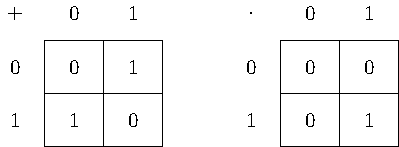
\includegraphics{ch1p25}
	\end{center}
	Check that properties P1-P9 all hold, even though $1 + 1 = 0$.
\end{problem}
